\documentclass[a4paper,12pt]{report}
\usepackage[utf8]{inputenc}
\usepackage[francais]{babel}
\usepackage{fancyhdr}
\usepackage{graphicx}
\usepackage{tikz}
\usetikzlibrary{calc}
\usepackage{listings}
\usepackage{xcolor}
\definecolor{grey}{rgb}{0.9,0.9,0.9}
\usepackage{titlesec}
\usepackage{verbatim}
\usepackage{listings}
\usepackage{textcomp}
\usepackage{hyperref}
\usepackage{amssymb}
\usepackage{amsmath}
\usepackage{longtable}
\usepackage{colortbl}
\usepackage{float}
\usepackage{caption}
\usepackage{subfig}
\usepackage{color}


\lstset{ %
  language=R,                     % the language of the code
  basicstyle=\footnotesize,       % the size of the fonts that are used for the code
  numbers=left,                   % where to put the line-numbers
  numberstyle=\tiny\color{gray},  % the style that is used for the line-numbers
  stepnumber=1,                   % the step between two line-numbers. If it's 1, each line
                                  % will be numbered
  numbersep=5pt,                  % how far the line-numbers are from the code
  backgroundcolor=\color{white},  % choose the background color. You must add \usepackage{color}
  showspaces=false,               % show spaces adding particular underscores
  showstringspaces=false,         % underline spaces within strings
  showtabs=false,                 % show tabs within strings adding particular underscores
  frame=single,                   % adds a frame around the code
  rulecolor=\color{black},        % if not set, the frame-color may be changed on line-breaks within not-black text (e.g. commens (green here))
  tabsize=2,                      % sets default tabsize to 2 spaces
  captionpos=b,                   % sets the caption-position to bottom
  breaklines=true,                % sets automatic line breaking
  breakatwhitespace=false,        % sets if automatic breaks should only happen at whitespace
  title=\lstname,                 % show the filename of files included with \lstinputlisting;
                                  % also try caption instead of title
  keywordstyle=\color{blue},      % keyword style
  commentstyle=\color{green},   % comment style
  stringstyle=\color{magenta},      % string literal style
  escapeinside={\%*}{*)},         % if you want to add a comment within your code
  morekeywords={*,...}            % if you want to add more keywords to the set
} 


\frenchbsetup{StandardLists=true}
\newcommand{\marge}{18mm}
\usepackage[left=\marge,right=\marge,top=\marge,bottom=\marge]{geometry}
\pagestyle{fancy}
\setlength{\headheight}{14pt}
\chead{
  \textbf{Binôme :} Douaille Erwan \& François Rémy
  \hspace{2em}
  \textbf{Groupe :} M1 Info RDF}
\renewcommand{\headrulewidth}{1pt}
\linespread{1}
\setlength{\columnseprule}{0.2pt}





\begin{document}


\makeatletter
\begin{titlepage}
\centering
\vspace{-10em}
{\LARGE \textbf{\textsc{Rapport de Projet RVI}}}\\
\vspace{3em}

\includegraphics[scale=0.6]{image/thalassa.png}\\
\vspace{3em}
{\LARGE \textsc{Projet Thalassa: simulation de plongée sous-marine}}\\

\vspace{8em}
Par\\
\vspace{1em}
{\LARGE \@author}\\

\vspace{2em}



\begin{tikzpicture}[remember picture,overlay]

\node [below left,xshift=-1cm, yshift=4cm] at (current page.south east){
\includegraphics[scale=0.6]{image/ustl1.png}};

\end{tikzpicture}
\end{titlepage}
\makeatother

\sloppy

\setcounter{page}{1} 
\newpage

%%%%%%%%%%%%%%%%%%%%%%%%%%%%%%%%%%%% INTRODUCTION
%%%%%%%%%%%%%%%%%%%%%%%%%%%%%%%%%%%%%%%%%%%%%%%%%
%%%%%%%%%%%%%%%%%%%%%%%%%%%%%%%%%%%%%%%%%%%%%%%%%
\section*{Introduction}

Le but du TP est d'utiliser l'outil de clustering kmeans pour classifié automatiquement des données sans utiliser de méthode d'apprentissage.
	
\section*{Question 1}

\begin{lstlisting}
	library(MASS)
library(mclust)

#Q1
(load(file="iris-tp8.RData"))
couleur <- rep('red', n)
couleur[classe==2]='green'
couleur[classe==3]='blue'

# run K-Means
km1 <- kmeans(x, 3, 15)
km2 <- kmeans(x, 3, 15)
km3 <- kmeans(x, 3, 15)
km4 <- kmeans(x, 3, 15)
km5 <- kmeans(x, 3, 15)
print(x_aff)
# plot centers
centers_aff <- cbind(km5$centers[,2],km5$centers[,4])
shape<-rep(1, n) 
shape[classe==2]=2
shape[classe==3]=3
plot(x_aff, col=couleur,pch=shape)
points(centers_aff, col = 'black', pch = 8)
print("Taux erreur:")
print(classError(km5$cluster, classe))
\end{lstlisting}


\begin{figure}[!ht]
	\center
	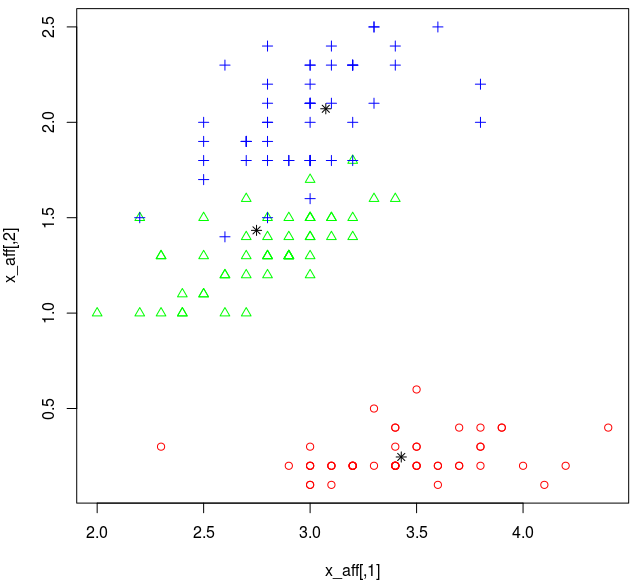
\includegraphics[scale=0.3]{image/q1.png}
\end{figure}


\begin{tabular}{|c|c|c|c|c|c|c|c|}
   \hline
   \cellcolor{gray!40}\textbf{Éxécution} & \cellcolor{gray!40}\textbf{Taux erreur} & \multicolumn{2}{c}{\cellcolor{gray!40}\textbf{Centre gravité 1}} & \multicolumn{2}{c}{\cellcolor{gray!40}\textbf{Centre gravité 2}} & \multicolumn{2}{c}{\cellcolor{gray!40}\textbf{Centre gravité 3}} \\
   \hline
   \cellcolor{gray!40}\textbf{ } & \cellcolor{gray!40}\textbf{ } & 		\cellcolor{gray!40}\textbf{x}& 		\cellcolor{gray!40}\textbf{y}& 		\cellcolor{gray!40}\textbf{x}& 		\cellcolor{gray!40}\textbf{y}& 		\cellcolor{gray!40}\textbf{x}& 		\cellcolor{gray!40}\textbf{y} \\
   \hline
   1 & 0.333 & 3.624242 & 0.2727273 & 2.895833  & 1.7031250 & 2.904762 & 0.3523810  \\
   \hline
   2 & 0.10666 & 2.748387 & 1.433871 & 3.428000 & 0.246000 & 3.073684 & 2.071053  \\
   \hline
   3 & 0.10666 & 2.748387 & 1.433871 & 3.428000 & 0.246000 & 3.073684 & 2.071053 \\
   \hline
   4 & 0.10666 & 3.073684 & 2.071053 & 3.428000 & 0.246000 & 2.748387 & 1.433871 \\
   \hline
   5 & 0.10666 & 3.428000 & 0.246000 & 2.748387 & 1.433871 & 3.073684 & 2.071053 \\
   \hline
\end{tabular}

On observe que le taux d'erreur change de la première à la deuxième éxécution et reste ensuite fixe. Concernant les centres de gravité on observe de grandes différences sur les positions, notamment sur l'axe des ordonnée. À chaque itération on affine la position des centres de gravité de chaque classe, plus on fait d'itération plus on aura un centre de gravité précis.

\newpage

\section*{Question 2}

\begin{lstlisting}library(MASS)
library(mclust)
(load(file="iris-tp8.RData"))
couleur <- rep('red', n)
couleur[classe==2]='green'
couleur[classe==3]='blue'
centre_init <- t(matrix(c(x[1,],x[51,],x[101,]),4,3));
km5 <- kmeans(x, 3, 15, centers = centre_init)
print(x_aff)
# plot centers
centers_aff <- cbind(km5$centers[,2],km5$centers[,4])
shape<-rep(1, n) 
shape[classe==2]=2
shape[classe==3]=3
plot(x_aff, col=couleur,pch=shape)
points(centers_aff, col = 'black', pch = 8)
print("Taux erreur:")
print(classError(km5$cluster, classe))
\end{lstlisting}


\begin{figure}[!ht]
	\center
	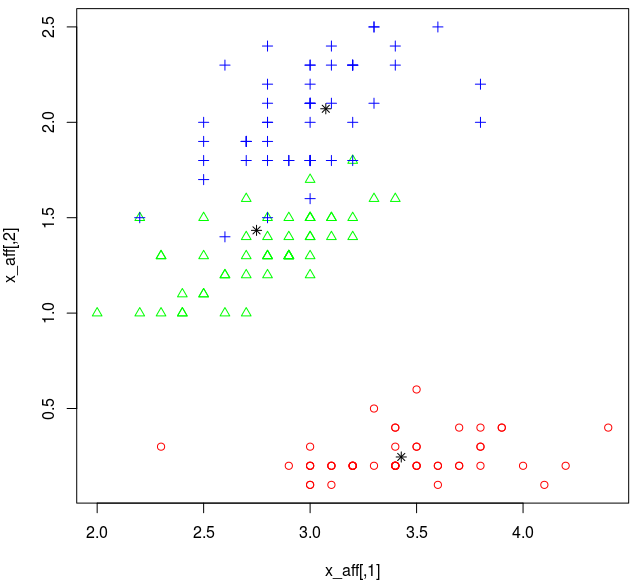
\includegraphics[scale=0.3]{image/q1.png}
\end{figure}


\begin{tabular}{|c|c|c|c|c|c|c|c|}
   \hline
   \cellcolor{gray!40}\textbf{Éxécution} & \cellcolor{gray!40}\textbf{Taux erreur} & \multicolumn{2}{c}{\cellcolor{gray!40}\textbf{Centre gravité 1}} & \multicolumn{2}{c}{\cellcolor{gray!40}\textbf{Centre gravité 2}} & \multicolumn{2}{c}{\cellcolor{gray!40}\textbf{Centre gravité 3}} \\
   \hline
   \cellcolor{gray!40}\textbf{ } & \cellcolor{gray!40}\textbf{ } & 		\cellcolor{gray!40}\textbf{x}& 		\cellcolor{gray!40}\textbf{y}& 		\cellcolor{gray!40}\textbf{x}& 		\cellcolor{gray!40}\textbf{y}& 		\cellcolor{gray!40}\textbf{x}& 		\cellcolor{gray!40}\textbf{y} \\
   \hline
   1 & 0.10666 & 3.428000 & 0.246000 & 2.748387 & 1.433871 & 3.073684 & 2.071053 \\
   \hline
\end{tabular}\\

En supprimant l'initialisation aléatoire en ajoutant le centre$\_$init on obtient directement un taux d'erreur de valeur 0.10667. Les centres de gravité sont correctement initialisés comme à l'itération 5 de la question précédente.


\newpage

\section*{Question 3}

\begin{lstlisting}
library(MASS)
library(mclust)

(load(file="iris-tp8.RData"))
couleur <- rep('red', n)
couleur[classe==2]='green'
couleur[classe==3]='blue'

# ACP
S <- cov(x_aff)
Vp <- eigen(S)  

pente <- Vp$vectors[2,1]/Vp$vectors[1,1]
ScalarProduct <- x_aff * (Vp$vectors[,1]) / sqrt(sum(Vp$vectors[,1]*Vp$vectors[,1]));
XP <- x_aff
XP[,1] = ScalarProduct * Vp$vectors[1,1]
XP[,2] = ScalarProduct * Vp$vectors[2,1]

centre_init <- t(matrix(c(XP[1,],XP[51,],XP[101,]),2,3));
km5 <- kmeans(XP, 3, 15, centers = centre_init)
print(XP)
# plot centers
centers_aff <- cbind(km5$centers[,1],km5$centers[,2])
shape<-rep(1, n) 
shape[classe==2]=2
shape[classe==3]=3
print("Taux erreur:")
print(classError(km5$cluster, classe))

plot(x_aff, col=couleur,pch=shape, xlim=c(-1,5), ylim=c(-2,3))
abline(a = 0, b = pente, col = "black")
points(XP[classe==1,], col="red")
points(XP[classe==2,], col="green")
points(XP[classe==3,], col="blue")
points(centers_aff, col = 'black', pch = 8)
\end{lstlisting}


\begin{figure}[!ht]
	\center
	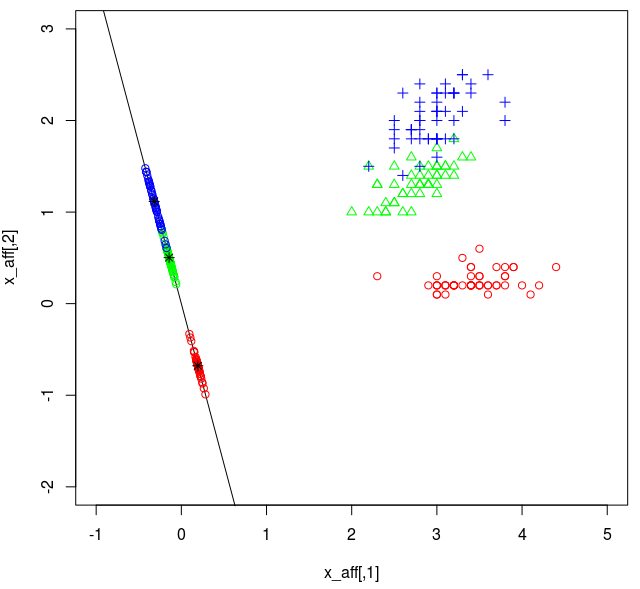
\includegraphics[scale=0.3]{image/q3.png}
\end{figure}
\begin{center}

\begin{tabular}{|c|c|c|c|c|c|c|c|}
   \hline
   \cellcolor{gray!40}\textbf{Éxécution} & \cellcolor{gray!40}\textbf{Taux erreur} & \multicolumn{2}{c}{\cellcolor{gray!40}\textbf{Centre gravité 1}} & \multicolumn{2}{c}{\cellcolor{gray!40}\textbf{Centre gravité 2}} & \multicolumn{2}{c}{\cellcolor{gray!40}\textbf{Centre gravité 3}} \\
   \hline
   \cellcolor{gray!40}\textbf{ } & \cellcolor{gray!40}\textbf{ } & 		\cellcolor{gray!40}\textbf{x}& 		\cellcolor{gray!40}\textbf{y}& 		\cellcolor{gray!40}\textbf{x}& 		\cellcolor{gray!40}\textbf{y}& 		\cellcolor{gray!40}\textbf{x}& 		\cellcolor{gray!40}\textbf{y} \\
   \hline
   1 & 0.033333 & 0.1936962 & -0.6780002 & -0.1436179 & 0.5027096 & -0.3188237 & 1.1159874 \\
   \hline
\end{tabular}\\
\end{center}

Avec cette méthode, on observe que le taux d'erreur est plus faible et le centre de gravité est parfaitement sur la droite de projection. Chaque classe à son point de gravité plus ou moins au centre de l'ensemble de ses points sur la droite de projection. On observe donc que la droite de projection nous à permis de mieux determiner les classes et de mieux placer le centre de gravité de chacune de ces classes.

\newpage

\section*{Conclusion}
Nous pouvons en conclure que l'utilisation de la méthode des kmeans nous permet d'avoir un reconnaissance sans intervention extérieure (mode non supervisé). De plus nous obtenons des taux d'erreur relativement faibles. Couplé à une analyse en composantes principales, le taux d'erreur devient encore plus faible et nous obtenons une distinction des formes très bonne.

\end{document}

